\subsection{bpmanalysis/bpm\_\-analysis.h File Reference}
\label{bpm__analysis_8h}\index{bpmanalysis/bpm\_\-analysis.h@{bpmanalysis/bpm\_\-analysis.h}}


\subsubsection{Detailed Description}
libbpm analysis routines 

This header contains definitions for the libbpm BPM data analysis routines. These mainly are the SVD and resolution/residual calculation routines along with the definition of an analysis cut function... 

Definition in file {\bf bpm\_\-analysis.h}.

{\tt \#include $<$math.h$>$}\par
{\tt \#include $<$bpm/bpm\_\-defs.h$>$}\par
{\tt \#include $<$bpm/bpm\_\-interface.h$>$}\par


Include dependency graph for bpm\_\-analysis.h:\nopagebreak
\begin{figure}[H]
\begin{center}
\leavevmode
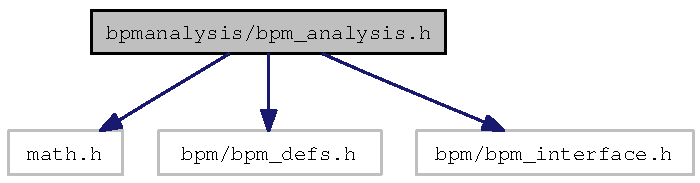
\includegraphics[width=186pt]{bpm__analysis_8h__incl}
\end{center}
\end{figure}
\subsubsection*{Defines}
\begin{CompactItemize}
\item 
\#define {\bf BPM\_\-GOOD\_\-EVENT}
\item 
\#define {\bf BPM\_\-BAD\_\-EVENT}
\item 
\#define {\bf ANA\_\-SVD\_\-TILT}
\item 
\#define {\bf ANA\_\-SVD\_\-NOTILT}
\end{CompactItemize}
\subsubsection*{Functions}
\begin{CompactItemize}
\item 
EXTERN int {\bf ana\_\-set\_\-cutfn} (int($\ast$cutfn)({\bf bpmproc\_\-t} $\ast$proc))
\item 
EXTERN int {\bf ana\_\-get\_\-svd\_\-coeffs} ({\bf bpmproc\_\-t} $\ast$$\ast$proc, int num\_\-bpms, int num\_\-svd, int total\_\-num\_\-evts, double $\ast$coeffs, int mode)
\item 
EXTERN int {\bf ana\_\-compute\_\-residual} ({\bf bpmproc\_\-t} $\ast$$\ast$proc, int num\_\-bpms, int num\_\-evts, double $\ast$coeffs, int mode, double $\ast$mean, double $\ast$rms)
\item 
EXTERN int {\bf ana\_\-def\_\-cutfn} ({\bf bpmproc\_\-t} $\ast$proc)
\end{CompactItemize}
\subsubsection*{Variables}
\begin{CompactItemize}
\item 
EXTERN int($\ast$ {\bf ana\_\-cutfn} )({\bf bpmproc\_\-t} $\ast$proc)
\end{CompactItemize}
